% PDF 78
\sourcepage{74}{78}
即从 $\mathfrak X_A$ 到 $k$ 上仿射直线的态射。由于 $\mathbb E^1$ 由单变量多项式环 $k[T]$ 表示，将两个互为反范畴的范畴中的箭头反向，就得到集合之间的双射
\begin{equation}\tag{5.3}
\Hom_{\Aff_k}(\mathfrak X_A,\mathbb E^1)
\simeq\Hom(k[T],A)\simeq A.
\end{equation}
这里最后一个双射来自如下事实：任一 $k$-代数同态 $u:k[T]\to A$ 都由 $u(T)\in A$ 唯一确定；反过来，对任意 $a\in A$，都恰有一个 $u$ 满足 $u(T)=a$。换言之，从集合 (5.2) 可以恢复 $A$ 的底集。再回忆一下，$\mathbb E^1$ 正是将每个 $k$-代数 $k'$ 映到其底集的遗忘函子。而 $k'$ 具有 $k$-代数结构，因此函子 $\mathbb E^1$ 本身也带有 $k$-代数结构。\footnote{Grothendieck 在这里引用了他此前的讲义，见 AAG。读者也可参阅 Dieudonné，\textit{Advances}，II，第 420 页，或 EGA-Springer，\S 0.6，第 41 页。}

\Section{6}{$\Aff_k$ 中的纤维积与核}
\textbf{提要。} $\Aff_k$ 中任意类型的逆极限，都与其反范畴 $\G_k$ 中相应的归纳极限一一对应（参见第 3 节）。\footnote{嵌入 $i:C\hookrightarrow\widehat C$（见第一章第 1 节）把任意 $\mathfrak X_A\in\Ob C$ 看成从 $C$ 到集合范畴的反变函子，等价地，看成从 $\G_k$ 到集合范畴的协变函子：$k'\mapsto\Hom_{k\text{-alg}}(A,k')$，$k'\in\G_k$。纯粹从范畴论来看，$i$ 与逆极限相容（见第 2 节）。也就是说，给定 $C$ 中的一个图式，在 $\widehat C$ 中总存在逆极限 $\varprojlim i(X_\alpha)$；当且仅当它可表时，我们说它属于 $C$。此时，$C$ 中的逆极限可定义为任一表示对象，因而在同构意义下唯一。这里的重要结论是：$C$ 中任意图式在 $\widehat C$ 中的逆极限始终可表。对偶地，$k$-代数范畴中存在任意类型的归纳极限。}
根据第 2 节的化归，只需证明下列两组结论中的任意一组：
\begin{enumerate}[label=\arabic*)]
\item $\Aff_k$ 中存在任意积，包括终对象 $\mathfrak X_k$；并且，对任意一对态射 $X\to S$、$Y\to S$，纤维积 $X\times_S Y$ 存在。
\item $\Aff_k$ 中存在任意积，以及任意一对态射 $\mathfrak X_A\rightrightarrows\mathfrak X_B$ 的核。
\end{enumerate}
由对偶性，只需验证 $\G_k$ 中存在任意余积（和、合并和），以及任意一对箭头 $B\rightrightarrows A$ 的余核。对具备适当交换代数知识的读者，这两项验证都很直接。有限和总可以化归到两个 $k$-代数 $A,B$ 的情形；它们在 $\G_k$ 中的范畴和，就是

% PDF 79
\sourcepage{75}{79}
张量积 $A\otimes_k B$。更一般地，对于任意一族 $k$-代数，都可以定义 $\bigotimes_{\alpha\in I,k} A_\alpha$。另一方面，一对箭头 $u,v:B\rightrightarrows A$ 的余核，由典范满射 $k$-代数同态 $A\to A/\mathfrak J$ 给出，其中
\[
\mathfrak J=\bigl(\,u(b)-v(b)\mid b\in B\,\bigr)
\]
是由这些差所生成的 $A$ 的理想。

设 $\{X_\alpha\}_{\alpha\in I}$ 是由集合 $I$（未必有限）指标的一族仿射代数空间，$X_\alpha\in\Ob C$。则积 $\prod_{\alpha\in I}X_\alpha$ 总能在 $C$ 中定义，且在同构意义下唯一（参见第 1 节）。这等价于说：

\textbf{在 $k$-代数范畴 $\G_k$ 中，任意一族对象的和总是存在；确切地说，它就是张量积 $\bigotimes_{\alpha\in I,k}A_\alpha$。}

换言之，设 $X_\alpha=\mathfrak X_{A_\alpha}$（$\alpha\in I$），即 $X_\alpha$ 是由 $k$-代数 $A_\alpha\in\Ob\G_k$ 表示的仿射代数空间。则 $\prod_{\alpha\in I}X_\alpha$ 由张量积表示：
\begin{equation}\tag{6.1}
\prod_{\alpha\in I}\mathfrak X_{A_\alpha}=\mathfrak X_A,
\qquad A=\bigotimes_{\alpha\in I,k}A_\alpha,
\end{equation}
因为 $A$ 是这些 $A_\alpha$ 的范畴和（见第 3 节）。验证这一性质，只是把张量积熟知的泛性质换一种说法。\footnote{参见 Bourbaki，\textit{Linear Algebra}，第 3 节，第 76 页。}

为证明 $A$ 是范畴和，我们将说明下述嵌入（即「余投影」，参见第 3 节）$i_\alpha:A_\alpha\to A$（$\alpha\in I$），

% PDF 80
\sourcepage{76}{80}
\begin{equation}\tag{6.2}
i_\alpha(a)=1\otimes\cdots\otimes1\otimes\underset{\alpha}{a}\otimes1\otimes\cdots\otimes1
\qquad(a\in A_\alpha),
\end{equation}
\footnote{译注：原文公式 (6.2) 中将 $a$ 的所属集合写为 $A$；按 $i_\alpha$ 的定义，此处应为 $A_\alpha$。}具有和的熟知泛性质；这里每个 $\beta\ne\alpha$ 的位置上都是因子 $1$（见第 3 节）。

先考虑两个因子 $A'\otimes_k A''$（$A',A''\in\Ob C$）的和的性质。相应嵌入定义为
\[
a'\longmapsto a'\otimes_k1,
\qquad a''\longmapsto1\otimes_k a''.
\]
最后，当指标集 $I$ 无限时，注意到 $I$ 的有限子集 $I'\subset I$ 构成一个滤过正向系统。对每个有限的 $I'\subset I$，都可以定义
\[
A(I')=\bigotimes_{\alpha\in I',k}A_\alpha.
\]
而且，如果 $I'\subset I''\subset I$，其中 $I''$ 有限，就有诱导的 $k$-代数同态 $A(I')\to A(I'')$。于是可以定义
\[
A(I)=\varinjlim_{\substack{I'\subset I\\I'\text{ 有限}}}A(I').
\]
事实上，底集的归纳极限存在，且 $k$-代数结构能够传递到极限上。\footnote{关于代数的归纳极限，一个简短的介绍见 Atiyah--Macdonald 一书第 32--33 页习题 14。}

我们知道，对于 $\Aff_k$ 中任意一对态射 $X\xrightarrow f S$、$Y\xrightarrow g S$，纤维积 $X\times_S Y$ 的存在性（参见第 1 节），等同于这两个对象在范畴 $\Aff_k/S$ 中通常意义下的积的存在性。范畴 $\Aff_k/S$ 与 $\G_A$ 互为反范畴，其中 $A$ 是表示 $S$ 的 $k$-代数。事实上，设
\[
X=\mathfrak X_B,\qquad Y=\mathfrak X_C,\qquad S=\mathfrak X_A.
\]
则有 $k$-代数同态 $A\xrightarrow{f^*}B$、$A\xrightarrow{g^*}C$，方向分别与 $f,g$ 相反；它们与 $k$-代数结构相容，即给出交换图
\begin{equation}\tag{6.3}
\begin{tikzcd}[column sep=small,row sep=small,ampersand replacement=\&]
A\arrow[r,"f^*"]\&B\\
k\arrow[u]\arrow[ur]\&
\end{tikzcd}
\qquad
\begin{tikzcd}[column sep=small,row sep=small,ampersand replacement=\&]
A\arrow[r,"g^*"]\&C\\
k\arrow[u]\arrow[ur]\&
\end{tikzcd}
\end{equation}

% PDF 81
\sourcepage{77}{81}
其中竖直箭头是 $A$ 作为 $k$-代数的结构态射（参见第一章第 2 节）。于是 $B,C$ 都成为 $A$-代数，$X\times_S Y$ 存在，并由张量积 $B\otimes_A C$ 表示。也就是说：

\textbf{态射 $X\xrightarrow f S$、$Y\xrightarrow g S$ 的纤维积 $X\times_S Y$ 存在，且等于 $\mathfrak X_D$，其中 $D=B\otimes_A C$；这里 $B,C$ 的 $A$-代数结构由 $f^*,g^*$ 给出。}\footnote{读者只需把箭头反向，就能核实左边的纤维积图式如何由右边的张量积图式得到：
\[
\begin{tikzcd}[column sep=small,row sep=small,ampersand replacement=\&]
\&P\arrow[d,dashed]\&\\
\&X\times_S Y\arrow[dl]\arrow[dr]\&\\
X\arrow[dr,"f"']\&\&Y\arrow[dl,"g"]\\
\&S\&
\end{tikzcd}
\quad\longleftrightarrow\quad
\begin{tikzcd}[column sep=small,row sep=small,ampersand replacement=\&]
\&F\&\\
\&B\otimes_A C\arrow[u,dashed]\&\\
B\arrow[ur]\&\&C\arrow[ul]\\
\&A\arrow[ul,"f^*"]\arrow[ur,"g^*"']\&
\end{tikzcd}
\]}
前面两项验证，结合第 2 节中的第一种化归，就证明了 $\Aff_k$ 中存在任意逆极限。

还有另一种证明方法：对任意一对 $k$-代数箭头 $u,v:B\rightrightarrows A$，证明相应的一对态射 $\mathfrak X_A\rightrightarrows\mathfrak X_B$ 有核。也就是说，在 $\G_k$ 中构造 $u,v$ 的余核，即构造一个泛箭头 $A\xrightarrow w k'$（$k'\in\Ob\G_k$），使图
\begin{equation}\tag{6.4}
\begin{tikzcd}[ampersand replacement=\&]
B\arrow[r,shift left,"u"]\arrow[r,shift right,"v"']\&A\arrow[r,"w"]\&k'
\end{tikzcd}
\end{equation}
交换，即 $w\circ u=w\circ v$。这就是说，对每个 $b\in B$，都有 $w(u(b)-v(b))=0$。\footnote{译注：原文此句写为 $u(b)=v(b)$ 后推出 $w(u(b)-v(b))=0$；这里需要的是像在 $w$ 之下相等，即 $w(u(b))=w(v(b))$。}换言之，
\begin{equation}\tag{6.5}
u(b)-v(b)\in\Ker w\qquad(b\in B).
\end{equation}
反过来，$\G_k$ 中任何满足 (6.5) 的 $w$ 都使 (6.4) 交换。而 (6.5) 蕴涵
\[
\Ker w\supset\mathfrak J
=\bigl(\,u(b)-v(b)\mid b\in B\,\bigr).
\]
众所周知，$A/\mathfrak J$ 连同

% PDF 82
\sourcepage{78}{82}
典范满射同态 $A\xrightarrow p A/\mathfrak J$，正是所求的余核：对每个使 (6.4) 交换的 $w$，都能唯一补出下图中的虚线箭头，使图交换：
\begin{equation}\tag{6.6}
\begin{tikzcd}[ampersand replacement=\&]
B\arrow[r,shift left,"u"]\arrow[r,shift right,"v"']\&A\arrow[r,"p"]\arrow[d,"w"']\&A/\mathfrak J\arrow[dl,dashed]\\
\&k'\&
\end{tikzcd}
\end{equation}

\Section{7}{滤过逆极限；关于诺特环的补充讨论}
再给出最后一个逆极限的例子，这里 $C=\Aff_k$。设 $\{X_i\}_{i\in I}$（$X_i\in\Ob C$）是以滤过有序集 $I$（或滤过范畴）为指标的滤过逆向系统。当然，逆极限 $X=\varprojlim X_i$ 对应于 $k$-代数范畴 $\G_k$ 中的一个滤过归纳极限。我们要说明，在这个例子中，纯集合论的构造可以传递 $k$-代数结构：$A=\varinjlim_{i\in I}A_i$ 的底集，就是各个 $A_i$ 底集的归纳极限；正因为系统是滤过的，$k$-代数结构得以保留。

在代数几何中，这一构造常用于将任意 $k$-代数 $A$ 所表示的 $k$ 上仿射代数空间 $\mathfrak X_A$，化归到有限生成 $k$-代数的情形。具体来说，$\mathfrak X_A$ 是由各个 $\mathfrak X_{A_i}$ 组成的滤过逆向系统的逆极限，其中 $A_i$ 遍历 $A$ 的有限生成子代数。更确切地说，$A$ 是有限生成 $k$-子代数的滤过并：若 $A',A''$ 是 $A$ 的两个有限生成子代数，则由两者共同生成的子代数仍有限生成。\footnote{译注：原文写「它们的并仍有限生成」；两个子代数的集合并一般并非子代数，这里应理解为两者共同生成的子代数。}因此，由对偶性，$k$ 上的仿射代数空间 $\mathfrak X_A$ 是上述滤过

% PDF 83
\sourcepage{79}{83}
逆向系统 $\mathfrak X_{A_i}$ 的逆极限，其中 $A_i$ 遍历这些有限生成 $k$-子代数。

许多情形下，先在有限型情形证明的命题，可以通过取极限推广到一般情形。现在对 $k$ 上有限型的 $\mathfrak X_A$ 略作说明。

一个 $k$-代数 $A$ 称为 $k$ 上\textbf{有限型}（即在 $k$ 上有限生成），当且仅当
\[
A\simeq k[T_1,T_2,\ldots,T_n]/\mathfrak J,
\]
即 $A$ 同构于某个以 $k$ 为系数、含有限多个变量 $T_1,T_2,\ldots,T_n$ 的多项式环的商环。给出这样一个同构，等价于给出 $A$ 作为 $k$-代数的一组 $n$ 个生成元。换言之，$A$ 由一个多项式环连同一族方程 $f(T_1,\ldots,T_n)=0$（$f\in\mathfrak J$）描述；其中只须取理想 $\mathfrak J$ 的任意一组生成元。为了使 $k$ 上的代数 $A$ 的全部描述都由有限数据给出，最好要求 $\mathfrak J$ 有有限多个生成元。因此，如果 $A\simeq P_I/\mathfrak J$，其中 $I$ 有限且 $\mathfrak J$ 有限生成，就称 $A$ 是\textbf{有限表现的}。\footnote{容易作为习题证明：如果在一个表示 $A\simeq P_I/\mathfrak J$ 中，$\mathfrak J$ 有限生成，那么对任何另一个表示 $A\simeq P_{I'}/\mathfrak J'$（$I'$ 有限），$\mathfrak J'$ 也必有限生成。}

Hilbert 的另一个定理——基定理（\textit{Basissatz}）——告诉我们，在很多情形下，这样的多项式环 $k[T_1,T_2,\ldots,T_n]$ 的每个理想都是有限生成的；换言之，有限型代数已经是有限表现的。

% PDF 84
\sourcepage{80}{84}
确切地说：\textbf{若 $k$ 是域（经典情形中 $k=\mathbb R$ 或 $\mathbb C$），则 $k$ 上有限多个不定元的多项式环的每个理想都有限生成。}

如果一个环的每个理想都有限生成，就称它为\textbf{诺特环}。因此 Hilbert 基定理也可以表述为：域上的有限变量多项式环都是诺特环。\footnote{等价地，按 Emmy Noether 的说法，理想满足升链条件（a.c.c.）：诺特环 $A$ 的任意理想升链 $\mathfrak a_1\subset\mathfrak a_2\subset\cdots\subset\mathfrak a_n\subset\cdots$ 最终稳定，即存在 $m$ 使 $\mathfrak a_m=\mathfrak a_{m+1}=\cdots$；或者说，任何严格递增的理想链都是有限的。}

域 $k$ 当然是诺特环。$k[T]$ 是诺特环，则可由它是主理想整环这一事实得出。\footnote{但对于 $k[T_1,T_2]$，就较难直接看出这一点了。}
Hilbert 基定理还有一个更好的表述：

\textbf{如果 $k$ 本身是诺特环，那么 $k[T]$ 也是诺特环。}

参见 Bourbaki 或 Zariski--Samuel。由归纳法可知，如果 $k$ 是诺特环，那么 $k$ 上有限生成的代数，就是有限表现的代数。换言之，对每个由 $A\simeq k[T_1,\ldots,T_n]/\mathfrak J$ 表示的闭代数子空间 $X\hookrightarrow\mathbb E^n$，都可以用有限多个方程描述 $X$。\footnote{不过，Grothendieck 又一次表示，他不愿加上不必要的限制。$\mathfrak J$ 的一组典范生成元就是 $\mathfrak J$ 自身，而它很少是有限集！}

\Section{8}{$\Aff_k$ 中的归纳极限}
\textbf{Grothendieck 的提要。} 对于 $C=\Aff_k$ 中的归纳极限 $\varinjlim X_i$，我们知道它们对应于反范畴 $\G_k$ 中的逆极限 $\varprojlim A_i$，其中 $X_i=\mathfrak X_{A_i}$，$A_i\in\Ob\G_k$（$i\in I$）。这些逆极限在 $\G_k$ 中总是存在，因为各 $A_i$ 的底集的集合论

% PDF 85
\sourcepage{81}{85}
极限始终存在，而且代数结构可以传递到其上。困难出现在试图在反范畴 $C$ 中解释它们的时候：$C$ 中对偶的归纳极限往往不太符合几何直觉！例如，在 $\Aff_k$ 中取商会产生病态结果，因为它与在更一般的概形范畴中取商并不相同（参见第二卷）。\footnote{原因是，我们此前一直使用的方法，即将 $k$ 上仿射代数空间范畴 $C$ 嵌入从 $C$ 到集合范畴的反变函子范畴 $i:C\hookrightarrow\widehat C$，或等价地，嵌入从 $\G_k$ 到集合范畴的协变函子范畴，虽然与逆极限相容，却完全不与归纳极限相容。}

只有一种运算总是合理的：$k$ 上仿射代数空间范畴 $C$ 中的有限和运算 $\coprod_{i\in I}X_i$，其中指标集 $I=\{1,2,\ldots,n\}$ 有限。下面将详细描述它。

设 $X_i=\mathfrak X_{A_i}\in\Ob C$（$i\in I$）是有限多个 $k$ 上仿射代数空间，由 $k$-代数 $A_i$ 表示。我们要证明范畴和（即余积，见第 3 节）$\coprod_{i\in I}X_i$ 存在；这等价于反范畴 $\G_k$ 中有限积的存在性。事实上，这有限多个 $k$-代数的积 $A=\prod_{i\in I}A_i$ 就是范畴积，并且
\begin{equation}\tag{8.1}
\coprod_{i\in I}\mathfrak X_{A_i}=\mathfrak X_A,
\qquad A=\prod_{i\in I}A_i.
\end{equation}
即这 $n$ 个空间的和，由积 $k$-代数 $A$ 表示。\footnote{译注：原文此句作「这 $n$ 个 $k$-代数 $A_i$ 的和」，应指相应仿射代数空间的和；公式 (8.1) 已清楚给出了对应关系。}

来证明 $A=\prod_{i\in I}A_i$ 确实是这 $n$ 个 $k$-代数 $A_i$ 的范畴积。$A$ 的元素是有序 $n$ 元组 $(a_1,a_2,\ldots,a_n)$，其中 $a_i\in A_i$（$i=1,\ldots,n$）；加法和乘法按分量定义。$A$ 的单位元是 $(1,1,\ldots,1)$，其 $k$-代数结构由
\[
\lambda(a_1,a_2,\ldots,a_n)=(\lambda a_1,\lambda a_2,\ldots,\lambda a_n)
\qquad(\lambda\in k)
\]
给出，因而结构态射 $k\to A$ 为 $\lambda\mapsto(\lambda,\ldots,\lambda)$。单位元 $1$ 可分解成一组正交幂等元的和：

% PDF 86
\sourcepage{82}{86}
\begin{equation}\tag{8.2}
1=\sum_{i\in I}e_i,\qquad
 e_i^2=e_i=(0,\ldots,0,\underset{i}{1},0,\ldots,0),
\qquad e_ie_j=0\quad(i\ne j).
\end{equation}
存在 $n$ 个投影 $p_i:A\to A/A(1-e_i)\simeq A_i$（$i\in I$），其中 $A(1-e_i)$ 表示 $A$ 中由 $1-e_i$ 生成的理想。\footnote{另有集合意义下的嵌入 $a_i\mapsto(0,\ldots,a_i,\ldots,0)$，但它们不是 $\G_k$ 中的态射，因为 $A_i$ 的单位元被映到幂等元 $e_i$；当 $n>1$ 时，后者通常不是 $A$ 的单位元。}
对任意 $R\in\G_k$，都有双射
\begin{equation}\tag{8.3}
\Hom_{\G_k}(R,A)\simeq\prod_{i\in I}\Hom_{\G_k}(R,A_i).
\end{equation}

\textbf{评注。} 集合范畴中一族集合 $\{S_i\}_{i\in I}$ 的范畴和，就是它们的不交并 $\coprod_{i\in I}S_i$。于是自然要问：当 $k'\in\Ob\G_k$ 变化时，集合 $\mathfrak X_A(k')$ 是否就是各个 $\mathfrak X_{A_i}(k')$ 的不交并？即使在经典代数几何的框架中，也很容易构造反例。\footnote{设 $X,Y$ 是代数闭域 $k$ 上的不可约仿射代数簇，分别由整环 $A,B$ 表示。由 $A\times B$ 表示的 $X\amalg Y$，在 $k$-值点层面是 $X$ 与 $Y$ 的 $k$-值点的不交并。若 $I\subset X$、$J\subset Y$ 是不可约子簇，则 $I\amalg J$ 给出 $X\amalg Y$ 的一个 $k'$-值点，其中 $k'$ 是将 $A\times B$ 限制到 $I\amalg J$ 所得的 $k$-代数。
\[
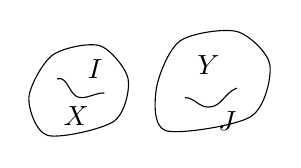
\begin{tikzpicture}[scale=.6]
\draw plot[smooth cycle] coordinates {(0,0)(-.4,.8)(.1,1.7)(1.1,1.9)(1.7,1.2)(1.4,.3)};
\draw plot[smooth cycle] coordinates {(2.5,.1)(2.3,1)(2.8,2)(4,2.2)(4.7,1.5)(4.3,.4)};
\draw (.2,1.2) to[out=15,in=180] (.7,.8) to[out=0,in=180] (1.2,.9);
\draw (2.9,.8) to[out=0,in=180] (3.4,.6) to[out=0,in=200] (4,1);
\node at (.6,.4){$X$};\node at (1,1.4){$I$};
\node at (3.4,1.5){$Y$};\node at (3.8,.3){$J$};
\end{tikzpicture}
\]}
对这一朴素想法的分析，引导 Grothendieck 研究 $\Aff_k$ 中的连通性概念。

现在来看看 $\mathfrak X_A$ 的 $k'$-值点（$k'\in\G_k$）究竟是什么样子。上面的满射 $A\to A_i$ 对应于单射 $\mathfrak X_{A_i}\hookrightarrow\mathfrak X_A$；简记 $X_i=\mathfrak X_{A_i}$、$X=\mathfrak X_A$，也就写成 $X_i\hookrightarrow X$。对每个 $k'$，都有单射 $X_i(k')\hookrightarrow X(k')$，从而给出由不交并到 $X(k')$ 的映射
\begin{equation}\tag{8.4}
\coprod_{i\in I}X_i(k')\longrightarrow X(k').
\end{equation}
问题在于：(8.4) 是否为同构？上面的脚注说明它未必如此。现在将这一情形与拓扑空间作一比较。\footnote{后面我们会把每个 $X_i\in\Ob\Aff_k$ 解释为带有一个环层的拓扑空间，因此这里的类比与所讨论的情形十分贴切。}
设在拓扑空间范畴中有拓扑空间的直和 $X=\coprod_{i\in I}X_i$，

% PDF 87
\sourcepage{83}{87}
其中 $X_i\in\Ob\mathcal T$。$X$ 是一个拓扑空间，各 $X_i$ 是其开子空间，它们两两不交且覆盖 $X$。因此，在集合意义下，$X$ 是各个 $X_i$ 的不交并；$X$ 上的拓扑则唯一地由下述要求确定：每个 $X_i$ 都是开集，且在 $X_i$ 上的诱导拓扑正是它原有的拓扑。换言之，$U\subset X$ 是开集，当且仅当对每个 $i\in I$，$U\cap X_i$ 都是 $X_i$ 中的开集。

另一方面，对任意拓扑空间 $Z$，有映射
\begin{equation}\tag{8.5}
\coprod_{i\in I}X_i(Z)\longrightarrow X(Z).
\end{equation}
\footnote{记号 $X(Z)$ 是 $\Hom_{\mathcal T}(Z,X)$ 的简写，即所有连续映射 $Z\to X$ 组成的集合。}
我们想知道 (8.5) 是否为双射。这意味着任意连续映射 $Z\to X$ 都恰好能通过某个 $X_i$ 作唯一的分解，即恰有一个指标 $i\in I$ 使下图交换：
\[
\begin{tikzcd}[column sep=small,ampersand replacement=\&]
Z\arrow[r]\arrow[d]\&X\\
X_i\arrow[ur,hook]\&
\end{tikzcd}
\]
如果 $Z$ 连通，这当然成立。但如果 $Z$ 含有多个连通分支，就可以把其中两个分别映入不同的 $X_i$，于是上述性质便不再成立。\footnote{可将这一陈述与原书第 II-8-3 页脚注 (2)，即上一原页中所述的经典代数几何情形作比较。}

回到 $\Aff_k$，我们预期，在这个范畴中，(8.5) 为双射恰好对应于 $Z$ 连通。这促使我们明确提出

% PDF 88
\sourcepage{84}{88}
$\Aff_k$ 中的连通性概念。

\textbf{连通性的范畴论定义。} 拓扑空间 $X$ 连通，当且仅当对任意和分解 $X=X'\amalg X''$（$X'\cap X''=\varnothing$），必有一个和项 $X'$ 或 $X''$ 是空集。回忆空集 $\varnothing$ 是 $\Sets$ 的始对象，就得到对任意范畴 $C$ 的如下推广。

对象 $X\in\Ob C$ 称为\textbf{连通的}，如果每当 $X$ 写成两个对象 $X',X''\in\Ob C$ 的和
\[
X=X'\amalg X'',
\]
总有 $X'$ 或 $X''$ 是 $C$ 的始对象。\footnote{空集 $\varnothing$ 也是拓扑空间范畴 $\mathcal T$ 的始对象。}

类比地，把 $\Aff_k$ 的始对象称为 $k$ 上的\textbf{空仿射代数空间}。它应由 $\G_k$ 的终对象表示。零环 $0$ 正是这样的对象，也就是空族 $k$-代数的积。\footnote{也就是说，对每个 $k$-代数 $k'$，都恰有一个同态 $k'\to0$。}

$\Aff_k$ 中的始对象 $\mathfrak X_0$，是把每个 $k$-代数 $k'$ 映到态射集 $\Hom(0,k')$ 的函子。如果 $k'\ne0$，即 $k'$ 中 $1\ne0$，这个集合就是空集；\footnote{注意，$\G_k$ 中的同态 $f:0\to k'$ 应满足 $f(0)=0_{k'}$、$f(1)=1_{k'}$，而在 $k'$ 中 $1\ne0$ 时，这是不可能的。}如果 $k'=0$，则它只有一个元素，即恒等态射。$\mathfrak X_0$ 就称为\textbf{空代数空间}。\footnote{不过，$\mathfrak X_0$ 并不是空函子。对任意 $A\in\Ob\G_k$，$\mathfrak X_A$ 都不会恒为空，因为 $\mathfrak X_A(A)$ 总含有恒等态射 $1_A:A\to A$。}

现在可以定义 $\Aff_k$ 中的连通性。$X=\mathfrak X_A$ 称为连通的，如果任意和分解 $X=X'\amalg X''$ 都迫使 $X'$ 或 $X''$ 为空代数空间；等价地，任意积分解

% PDF 89
\sourcepage{85}{89}
$A=A'\times A''$ 都迫使 $A'$ 或 $A''$ 为零 $k$-代数。从交换代数的角度看，这意味着什么？我们知道，把环 $A$ 分解为两个环 $A',A''$ 的积，等价于把单位元 $1\in A$ 分解为两个正交幂等元之和：\footnote{由于其熟知的几何意义，幂等元也常被称为投影元。}
\[
1=e'+e'',\qquad (e')^2=e',\qquad(e'')^2=e'',\qquad e'e''=0.
\]
\footnote{与前面类似，任何有限分解 $A=A_1\times\cdots\times A_n$，都等价于将 $1$ 分解成一组两两正交的幂等元 $e_i$ 之和。反过来，给定这样的分解，就能由 $A_i\simeq A/A(1-e_i)$（$i=1,\ldots,n$）恢复各个 $A_i$。}

我们稍微滥用一下术语，称 $A\in\Ob\G_k$ 是连通的，意即 $\mathfrak X_A$ 连通；这又等价于上述任何分解都是平凡的，即 $e'=0$ 或 $e''=0$。也就是说，每个幂等元只能是 $0$ 或 $1$。

\textbf{例。每个整环 $A$ 都是连通的。} 事实上，若 $e'\ne0$ 是幂等元，则 $1-e'$ 也是幂等元，且 $e'(1-e')=0$，从而 $1-e'=0$。

这个例子再次展示了整环与不可约性之间的熟知联系，这一联系早在「旧时代」的代数几何中就已经出现。
\begin{center}
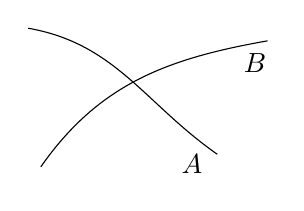
\begin{tikzpicture}[scale=.8]
\draw (-2,1) to[out=-10,in=145] (1,-1);
\draw (-1.8,-1.2) to[out=55,in=190] (1.8,.8);
\node at (.6,-1.15){$A$};\node at (1.6,.45){$B$};
\end{tikzpicture}
\end{center}
如果一个「代数簇」$X$ 能非平凡地分解为两个真子簇的并 $X=A\cup B$，就可以构造多项式函数 $f,g$，使 $f$ 在 $A$ 上恒为零而在 $B$ 上不恒为零，$g$ 在 $B$ 上恒为零而在 $A$ 上不恒为零。于是 $fg$ 在 $X$ 上为零，但 $f\ne0$、$g\ne0$。这样的「可约性」导致零因子的存在。在第三章第 5 节，我们会看到，古老的不可约性概念实际上是一个一般拓扑概念，而在 Zariski 拓扑中尤其具有表现力。

% PDF 90
\sourcepage{86}{90}
\BookChapter{3}{仿射概形}
第三章独立于第二章。在 EGA，I，第一章第 1 节第 79 页，Grothendieck 从仿射概形的定义开始建立代数几何；在逻辑上，这个定义并不以第一章的任何内容为前提。不过，第一章从多项式方程组出发，为后面的理论提供了很好的几何动机。

\textbf{Grothendieck 工作中最著名的一点，是以概形取代代数簇，作为代数几何的主要研究对象。最简单的概形是仿射概形；所有概形都由它们拼接而成（参见第二卷第五章）。}

仿射概形所起的作用，类似于仿射代数簇。事实上，Grothendieck 的定义受到 Serre 在 FAC 一文中以层论定义代数簇的启发。从逻辑上说，了解 FAC 并非必要；而把其中的内容收入这里，又会占去太多篇幅。由于 FAC 的相关内容，是 Grothendieck 在布法罗讲授的另一门课程——关于 Riemann--Roch--Grothendieck 定理的课程——的主要预备知识，我将在第二卷开头概述这套理论。

前面所用的几何语言，与可表函子 $\mathfrak X:\G_k\to\Sets$ 相联系；其中
\[
\mathfrak X(k')=V_A(k')=\Hom_{k\text{-alg}}(A,k')
\]
是 $k'$-值点的集合（$k'\in\Ob\G_k$，参见第一章）。现在我们要使用另一种几何语言：给函子 $\mathfrak X$（即 $V_A$）联系一个带有额外结构的拓扑空间，这就是所谓的仿射概形。这样做的一个原因在于，仿射概形使我们能够定义更一般的代数对象——概形。概形是把某些「仿射」部分，即仿射概形，粘合起来得到的。这一过程类似于从仿射代数簇这些仿射部分构造射影代数簇。射影代数簇，例如复射影代数簇，通常不能嵌入仿射空间。此外，还可以用其他方式把仿射代数簇或仿射概形粘合起来。我们需要建立一种把这些不同部分粘合起来的方法。最直观的方法之一，就是借助层论。因此，接下来要研究的是带有一个额外结构，即层 $\mathcal O_X$，的拓扑空间 $X$。

% PDF 91
\sourcepage{87}{91}
\textbf{提要。} $k$ 上的仿射代数空间函子 $\mathfrak X$，或者等价地，表示 $\mathfrak X=V_A$ 的 $k$-代数 $A$，有一个很大的不便：它并没有给 $A$ 配上一个单独的几何对象，而是给出一族随 $k'$ 变化的几何对象 $V_A(k')$。现在我们要给 $A$（因而也给 $\mathfrak X$）配上一个几何对象，即仿射概形 $(\Spec A,\widetilde A)$。\footnote{参见第一卷提要。$A$ 的谱 $\Spec A$ 是底拓扑空间，$\widetilde A$ 是其结构层。二元组 $(\Spec A,\widetilde A)$ 是一个局部赋环空间，因为 $\widetilde A$ 在各点的茎都是局部环。}
我们将分别研究拓扑空间 $X=\Spec A$ 及其结构层。$X$ 的谱拓扑（见第 2 节）可用 $A$ 的根理想 $\mathfrak a=\sqrt{\mathfrak a}$ 自然描述：$F\subset X$ 为闭集，当且仅当存在根理想 $\mathfrak a$，使得 $x\in F\Longleftrightarrow\mathfrak p_x\supset\mathfrak a$。\footnote{$\Spec A$ 的每个元素都有两种记法 $x,\mathfrak p_x$：将它看作 $\Spec A$ 中的点时写作 $x$，看作 $A$ 的素理想时写作 $\mathfrak p_x$。}
因而 $\Spec A=\Spec(A/\operatorname{Nil}A)$。因此，单凭 $X$ 无法恢复 $A$，除非将讨论限制在约化代数上，即 $\operatorname{Nil}A=0$，也就是 $0$ 是 $A$ 中唯一的幂零元。\footnote{译注：原文此处以约化情形说明丢失幂零信息的问题；即使限定为约化环，单凭谱的拓扑空间一般也不能恢复环，例如不同域的谱都是单点空间。后文引入结构层，才真正恢复环。}

为恢复 $A$，需要定义 $X$ 的\textbf{结构层} $\mathcal O_X=\widetilde A$。这样，$(X,\mathcal O_X)$ 就能给回 $A$：$A$ 同构于 $X$ 上整体截面所成的 $k$-代数，也就是零次上同调群，
\[
A\simeq\Gamma(X,\mathcal O_X)=H^0(X;\mathcal O_X).
\]
另一个有趣之处是，$k$ 在构造中并不占任何特殊地位；我们只用到了 $A$ 的含幺交换环结构。因此，函子 $A\mapsto(\Spec A,\widetilde A)$ 表明，由 $A$ 得到的仿射概形 $(\Spec A,\widetilde A)$ 可以与含幺交换环范畴 $\G$ 的反范畴 $\G^{\op}$ 的对象等同起来；同态 $A\xrightarrow f B$ 则对应于
\[
(\Spec B,\widetilde B)\xrightarrow{f^*}(\Spec A,\widetilde A).
\]

\PartTitle{第一部分}{函子 $\Spec:\G\to\mathcal T$}
\textbf{提要。} 本部分研究反变函子 $\Spec$：它从含幺交换环及保幺环同态所成的范畴 $\G$，映到拓扑空间及连续映射所成的范畴 $\mathcal T$。

集合 $\Spec A=\{\mathfrak p\mid\mathfrak p\text{ 是 }A\text{ 的素理想}\}$ 前面已经多次出现（见第一章原书第 10 页）。$\Spec A$ 上有一个自然的拓扑，称为 $A$ 的\textbf{谱拓扑}，也称 \textbf{Zariski 拓扑}，因为它是第一章第 14 节中所研究拓扑的自然内在版本。含幺交换环范畴 $\G$ 中的态射 $\varphi:A\to B$ 诱导映射
\begin{equation}\tag{0.1}
\Spec\varphi:\Spec B\longrightarrow\Spec A,
\end{equation}
这个映射是连续的。因此 $\Spec$ 是从 $\G$ 到拓扑空间及连续映射范畴 $\mathcal T$ 的反变函子。

% PDF 92
\sourcepage{88}{92}
第 1 节将说明这与第一章之间的联系，尽管直接作一个很初等的验证，也足以建立这一联系。

\Section{1}{$A$ 的处所与谱}
第一章第 8 节中，$A$ 的处所作为几何点的等价类而引入。相应的商集就是 $\Spec A$，也可以直接定义为 $A$ 的全体素理想所成的集合。

我们要说明，为何在构造 $\Spec A$、$\Max A$，乃至稍后引入 $A$ 的谱拓扑（见第 2 节）时，基环 $k$ 都没有任何特殊作用。设 $h:k\to A$ 是 $A$ 作为 $k$-代数的结构态射（$h\in\G$）。对 $\G$ 中任意态射 $A\xrightarrow f B$，只要取 $f\circ h$ 为结构态射，$B$ 就获得了一个确定的 $k$-代数结构。下面将取 $k=\mathbb Z$，也就是把 $\G$ 与 $\G_{\mathbb Z}$ 等同起来。

设 $\varphi:A\to B$ 是环同态，$\mathfrak b$ 是 $B$ 的任意理想。则有下列性质：
\begin{enumerate}[label=\arabic*)]
\item 逆像 $\varphi^{-1}(\mathfrak b)$ 是 $A$ 的理想。
\item 如果 $\mathfrak b$ 是素理想，则 $\varphi^{-1}(\mathfrak b)$ 也是 $A$ 的素理想。
\item 特别地，如果 $\mathfrak m$ 是 $B$ 的极大理想，则 $\varphi^{-1}(\mathfrak m)$ 是 $A$ 的素理想，但未必是极大理想；反例见下。
\end{enumerate}
验证留给读者。

性质 2) 表明，$\Spec$ 可以看作反变函子 $\G\to\Sets$；其中 $\Spec\varphi$（见 (0.1)）由 $\mathfrak b\mapsto\varphi^{-1}(\mathfrak b)$ 定义。请核实函子的性质！第 2 节将看到，在 $A,B$ 的谱上引入谱拓扑后，$\Spec\varphi$ 是连续的。换言之，

% PDF 93
\sourcepage{89}{93}
$\Spec$ 将被看作从 $\G$ 到拓扑空间及连续映射范畴 $\mathcal T$ 的反变函子。

\textbf{关于 $\Max(A)$ 的反例。} 设 $i:\mathbb Z\hookrightarrow\mathbb Q$ 是整数环到有理数域的自然包含。$\Max(\mathbb Q)=\Spec(\mathbb Q)=\{(0)\}$ 是仅含零理想的单点集。$i^{-1}(0)$ 是 $\mathbb Z$ 的零理想，因而属于 $\Spec(\mathbb Z)$：$\mathbb Z$ 的零理想是素理想，正因为 $\mathbb Z$ 是整环。但 $i^{-1}(0)$ 不是极大理想；对任意素数 $p>1$，都有严格包含 $(0)\subset(p)$。

正是这种函子性上的不良表现，使 Grothendieck 放弃用 $\Max A$ 作为各个 $\mathfrak X(k')$（$k'\in\Ob\G_k$）的某种内在替代物，尽管在 $k$ 是代数闭域，且 $\mathfrak X(k)$ 嵌入 $k^n$ 的经典情形中，确实可以在 $A$ 的极大理想与这个仿射模型的 $k$-值点之间建立一一对应。

\Section{2}{谱拓扑}
本节内容在 Bourbaki 的 \textit{Commutative Algebra}，1290，XXVII，第二章「局部化」第 3 节第 124 页中有详细论述。Grothendieck 在 EGA，I，IHES 中的原始论述，在 EGA-Springer 中被删去了；后者第一章第 1 节 1.1，第 194 页，只详细讨论了一些补充性质，直接从结构层开始。\footnote{其他不带证明的简短介绍，可见 Macdonald、Dieudonné 的 \textit{Advances I}，以及 Mumford 讲义；另参见 Lang、Atiyah--Macdonald。EGA-Springer 引言中从方程组出发的初等处理，在正文里没有采用，尽管在 EGA 中零散出现。我在其他地方只在 Manin 的 MTY 讲义中见过这种处理。}
本课程中，Grothendieck「起初」把 $A$ 看作基环 $k$ 上的代数。实际上，这一假设毫无限制性，因为每个 $A$ 都能借助唯一的结构态射 $\mathbb Z\to A$，看作 $\mathbb Z$-代数。

\textbf{提要。} 我们构造并研究从 $k$-代数范畴到拓扑空间范畴的反变函子 $\Spec$。拓扑空间 $X=\Spec A$ 的闭集 $Y$，可以刻画为任意方程组 $S:(f_i(u)=0)$ 的全体解的处所；但首先要赋予 $f_i(u)$ 一个内在的意义，说明其是否为零只依赖于 $A$ 的处所（见第一章第 8 节）。将证明：$S$ 可以取为由 $Y$ 唯一确定的根理想 $\mathfrak a=\sqrt{\mathfrak a}$。\footnote{这与经典情形一致：设 $k$ 是域，$A$ 是不含非零幂零元的有限生成 $k$-代数。如果 $A$ 是代数簇 $V$ 的多项式函数环，$W$ 是其子簇，那么 $W$ 上的多项式函数环，即限制 $B=A|_W$，由 $B=A/\mathfrak a$ 给出；这里 $\mathfrak a=\sqrt{\mathfrak a}$ 是所有在 $W$ 上为零的 $V$ 上函数组成的理想。归根结底，正是这个几何考虑决定了拓扑的选择。
\[
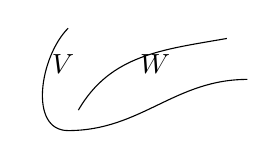
\begin{tikzpicture}[scale=.65]
\draw (0,2) to[out=225,in=180] (0,0) to[out=0,in=180] (3.5,1);
\draw (.2,.4) to[out=60,in=190] (3.1,1.8);
\node at (-.1,1.3){$V$};\node at (1.7,1.3){$W$};
\end{tikzpicture}
\]}
Grothendieck 去掉了此前对 $A$ 的种种限制，

% PDF 94
\sourcepage{90}{94}
特别是使 $k$ 退出了这一构造，同时说明所有本质性质依然成立。换言之，这个拓扑的闭集族完全可以用根理想描述。因而 $X=\Spec A$ 与 $\Spec(A/\operatorname{Nil}A)$ 同胚。子集 $Y\subset X$ 是闭集，当且仅当存在 $A$ 的某个根理想 $\mathfrak a=\sqrt{\mathfrak a}$，使 $Y$ 是 $\Spec(A/\mathfrak a)$ 在典范投影 $A\to A/\mathfrak a$ 所诱导映射下的像；参见原书第 89 页脚注 (2)。

$\Spec A$ 是 Kolmogorov 空间，即满足 $T_0$ 分离公理；但一般不满足 $T_1$，当然也更不满足 $T_2$（Hausdorff）条件，只有一些平凡情形例外。\footnote{$T_0$ 分离公理（Kolmogorov）：对任意两个不同的点 $x,y$，至少有一个点存在不含另一个点的开邻域，即存在开集 $U_x\ni x$、$y\notin U_x$，或存在开集 $U_y\ni y$、$x\notin U_y$。$T_1$ 分离公理（Fréchet）：对这样的 $x,y$，上述两种开邻域都存在。$T_1$ 等价于每个单点集 $\{x\}$ 都是闭集。$T_2$（Hausdorff）条件：存在分别包含 $x,y$ 的不相交开邻域 $U_x,U_y$，即 $U_x\cap U_y=\varnothing$。}
$\Spec A$ 是拟紧的。\footnote{拓扑空间 $X$ 称为拟紧的，是指任意开覆盖 $X=\bigcup_{i\in I}X_i$ 都有有限子覆盖。$X$ 紧，当且仅当它拟紧且 Hausdorff。本课程中出现的拓扑空间，除了一些平凡情形，一般都不是 Hausdorff 的。}

目前，$\Spec A$ 还只是一个集合：
\begin{equation}\tag{2.1}
X=\Spec A=\{\mathfrak p\mid\mathfrak p\text{ 是 }A\text{ 的素理想}\}.
\end{equation}
下面将描述 $X=\Spec A$ 在某个拓扑下的闭集族。这个拓扑称为 $X$ 的谱拓扑或 Zariski 拓扑（参见第一章第 14 节）。

对 $S=\{f_i\}_{i\in I}\subset A$，定义 $X$ 的子集
\begin{equation}\tag{2.2}
V(S)=\{\,u\in\mathfrak X(k')\text{ 的处所}\mid f_i(u)=0\text{ 对所有 }f_i\in S\,\}.
\end{equation}
这里 $\mathfrak X$ 是由 $A$ 表示的函子 $\G_k\to\Sets$，即 $A$ 所表示的 $k$ 上仿射代数空间；$u:A\to k'$ 是 $\mathfrak X$ 的一个几何点，也就是说，$k$-代数 $k'$ 是域（见第一章第 8 节）。\footnote{译注：原文将此 $\G_k\to\Sets$ 函子称为「反变」；按前文约定，它在 $k$-代数范畴上是协变的，在反范畴 $\Aff_k$ 上才是反变的。}

% PDF 95
\sourcepage{91}{95}
若 $f\in A$、$u\in\mathfrak X(k')$，定义 $f(u)\in k'$ 为
\begin{equation}\tag{2.3}
f(u)=u(f).
\end{equation}
于是 (2.2) 就有了意义，它表示 $u$ 满足「方程组」$\{f_i\}_{i\in I}$。

另一方面，(2.2) 与定义 $A$ 的处所的等价关系相容，即与代表元的选择无关，只依赖于处所。换言之，如果有 $k$-代数同态 $k'\to k''$，由于 $k',k''$ 是域，该同态必为单射；因此 $f_i(u)=0$ 等价于 $f_i(v)=0$，其中 $v$ 是 $u$ 在诱导映射下的像。而 $f_i(u)=u(f_i)=0$，正意味着 $f_i$ 属于 $u$ 的核。令 $\mathfrak p=\Ker u\in\Spec A$，便可看出 $V(S)$ 恰是包含 $S$ 的全体素理想所成的集合：
\begin{equation}\tag{2.4}
V(S)=\{x\in\Spec A\mid\mathfrak p_x\supset S\}.
\end{equation}
当然，$\mathfrak p\supset S$ 等价于 $\mathfrak p\supset\mathfrak J_S$，其中 $\mathfrak J_S$ 是由 $S$ 生成的理想。因此
\begin{equation}\tag{2.5}
V(S)=V(\mathfrak J_S).
\end{equation}
又因为素理想总等于其根，即 $\mathfrak p=\sqrt{\mathfrak p}$，把 $\mathfrak J_S$ 换成其根 $\sqrt{\mathfrak J_S}$，$V(S)=V(\mathfrak J_S)$ 仍不改变；也就是
\begin{equation}\tag{2.6}
V(S)=V(\mathfrak J_S)=V(\sqrt{\mathfrak J_S}).
\end{equation}
\footnote{这里避免用记号 $\widetilde{\mathfrak a}$ 表示根理想 $\sqrt{\mathfrak a}$，因为后面 $\widetilde A$ 将表示结构层。}
用文字来说，$A$ 中包含 $S$ 的素理想，恰好就是

% PDF 96
\sourcepage{92}{96}
包含由 $S$ 生成的理想 $\mathfrak J_S$ 的根 $\sqrt{\mathfrak J_S}$ 的素理想。

这一步已经不能再向前推进，因为可以用公式
\begin{equation}\tag{2.7}
\sqrt{\mathfrak J}=\bigcap_{x\in V(\mathfrak J)}\mathfrak p_x
\end{equation}
从 $V(\sqrt{\mathfrak J})$ 恢复 $\sqrt{\mathfrak J}$。这正是因为 $\sqrt{\mathfrak J}$ 等于 $A$ 中所有包含 $\mathfrak J$ 的素理想之交。\footnote{可借助典范映射 $A\to A/\mathfrak J=B$，把下述性质「提升到 $A$」来说明：$\operatorname{Nil}B$，即 $B$ 的全体幂零元，等于 $B$ 的全体素理想之交。}

由此证明了如下性质：

\textbf{能写成 $V(S)$ 形式的集合，恰好就是形如 $V(\mathfrak J)$、其中 $\mathfrak J=\sqrt{\mathfrak J}$ 的集合；而 $\mathfrak J$ 可以由 $V(\mathfrak J)$ 通过公式 (2.7) 恢复。}

换言之，$\Spec A$ 中能写成 $V(S)$ 形式的集合——以下称为 $X$ 的\textbf{代数子集}——与 $A$ 的根理想一一对应，且对应关系反转包含关系。例如，若 $\mathfrak J=\sqrt{\mathfrak J}$、$\mathfrak a=\sqrt{\mathfrak a}$，则
\[
\mathfrak J\subsetneq\mathfrak a\quad\Longrightarrow\quad
V(\mathfrak a)\subsetneq V(\mathfrak J).
\]

现在考察这些代数子集在取并与取交时的表现，为此写下两个公式 (2.8)、(2.9)。首先，
\begin{equation}\tag{2.8}
\bigcap_{i\in I}V(\mathfrak a_i)
=V\Bigl(\bigcup_{i\in I}\mathfrak a_i\Bigr)
=V\Bigl(\sum_{i\in I}\mathfrak a_i\Bigr).
\end{equation}
也就是说，$\Spec A$ 的任意一族代数子集之交，仍是 $\Spec A$ 的代数子集。

再看有限并，有

% PDF 97
\sourcepage{93}{97}
\begin{equation}\tag{2.9}
V\Bigl(\prod_{1\le i\le n}\mathfrak a_i\Bigr)
=\bigcup_{1\le i\le n}V(\mathfrak a_i).
\end{equation}
(2.8) 很明显。(2.9) 可如下证明。首先，由每个包含关系 $\prod_{1\le i\le n}\mathfrak a_i\subset\mathfrak a_i$，得到反向的包含 $V(\prod_{1\le i\le n}\mathfrak a_i)\supset V(\mathfrak a_i)$，所以
\begin{equation}\tag{2.10}
V\Bigl(\prod_{1\le i\le n}\mathfrak a_i\Bigr)
\supset\bigcup_{1\le i\le n}V(\mathfrak a_i).
\end{equation}
反过来，要证明 $x\in V(\prod_{1\le i\le n}\mathfrak a_i)$ 蕴涵对某个 $i$ 有 $x\in V(\mathfrak a_i)$。否则，对每个 $i=1,\ldots,n$，都有 $\mathfrak p_x\not\supset\mathfrak a_i$，于是可取 $f_i\in\mathfrak a_i$ 而 $f_i\notin\mathfrak p_x$。但 $f_1f_2\cdots f_n\in\mathfrak p_x$，这与 $\mathfrak p_x$ 是素理想矛盾。

显然还有
\begin{equation}\tag{2.11}
\varnothing=V(A),\qquad X=V(0)=V(\operatorname{Nil}A).
\end{equation}
结合前面的讨论，可知由 $V(\mathfrak J)$（$\mathfrak J=\sqrt{\mathfrak J}$）组成的集合族含有 $\varnothing$ 和 $X$，并且对任意交和有限并封闭。换言之：

\textbf{集合族 $V(\mathfrak J)$，其中 $\mathfrak J$ 遍历 $A$ 的根理想，满足 $X=\Spec A$ 上拓扑的闭集公理。}
这一拓扑称为 $X=\Spec A$ 的\textbf{谱拓扑}或 \textbf{Zariski 拓扑}。以下用 $\Spec A$ 表示相应的拓扑空间。

现在证明 $X$ 拟紧。\footnote{定义见原书第 III-2-2 页，即原书第 90 页的脚注。}
也就是说，如果 $X=\bigcup_{i\in I}U_i$，其中各 $U_i$ 都是开集，$I$ 任意，则必有有限子族覆盖 $X$。用闭集来表达，这等价于：如果 $(Y_i)_{i\in I}$ 是任意

% PDF 98
\sourcepage{94}{98}
一族闭集，且 $\bigcap_{i\in I}Y_i=\varnothing$，则其中已有有限个闭集的交为空。取 $A$ 的理想 $\mathfrak a_i$，使 $Y_i=V(\mathfrak a_i)$。令这些理想的和为 $\mathfrak a=\sum_{i\in I}\mathfrak a_i$，则 $V(\mathfrak a)=\varnothing$；这等价于 $\mathfrak a$ 不包含于任何素理想。对 $A/\mathfrak a$ 应用 Krull 定理——任何非零含幺环都至少有一个极大理想，因而至少有一个素理想——可知，除非 $\mathfrak a=A$，否则 $\mathfrak a$ 总包含于某个素理想。换言之，
\begin{equation}\tag{2.12}
V(\mathfrak a)=\varnothing\quad\Longleftrightarrow\quad\mathfrak a=A.
\end{equation}
因此 $\sum_{i\in I}\mathfrak a_i=A$，于是可以写成 $1=\sum_{i\in I}f_i$，其中 $f_i\in\mathfrak a_i$，且只有有限多个 $f_i$ 非零。这意味着有限多个 $\mathfrak a_i$ 的和已等于 $A$，也就是说，相应有限多个 $Y_i$ 的交为空！

来考察单点集 $\{x\}$ 在 $X$ 中的闭包 $\overline{\{x\}}$。它是包含 $x$ 的最小闭子集。设 $Y=V(\mathfrak a)$，则 $x\in Y$ 等价于 $\mathfrak a\subset\mathfrak p_x$。因此，包含 $x$ 的最小闭集，对应于包含在 $\mathfrak p_x$ 中的最大理想 $\mathfrak a$，也就是 $\mathfrak p_x$ 自身。故
\begin{equation}\tag{2.13}
y\in\overline{\{x\}}\quad\Longleftrightarrow\quad\mathfrak p_y\supset\mathfrak p_x.
\end{equation}
因此，\textbf{特化关系} $y\in\overline{\{x\}}$ 对应于素理想之间的反向包含关系。\footnote{设 $x,y$ 是任意拓扑空间 $X$ 的两个点。如果 $y\in\overline{\{x\}}$，就称 $y$ 是 $x$ 的一个特化，参见下节。在任何 $T_1$ 空间，特别是在 Hausdorff 空间中，$y$ 是 $x$ 的特化就意味着 $y=x$，因而这个概念变得平凡。}

\textbf{推论。} 1) 单点集 $\{x\}$ 是闭集，当且仅当素理想 $\mathfrak p_x$ 是极大理想。

% PDF 99
\sourcepage{95}{99}
2) $X$ 是 $T_1$ 空间，即 $X$ 的每一点都是闭点，当且仅当 $A$ 的每个素理想都是极大理想。

含有非极大素理想的环有很多，因此 $X$ 未必是分离空间！下面马上来验证 $T_0$ 公理，参见原书第 III-2-2 页脚注 (*)。

若 $y\in\overline{\{x\}}$，则每个包含 $x$ 的闭集也都包含 $y$；等价地，$y$ 的每个开邻域都包含 $x$。

设 $Y$ 是拓扑空间 $X$ 的一个不可约子集。$Y$ 中的点 $g$ 称为 $Y$ 的\textbf{一般点}，如果满足下列两个等价条件之一：
\begin{enumerate}[label=\arabic*)]
\item $Y=\overline{\{g\}}$；也就是说，每个包含 $g$ 的闭集，都包含 $Y$ 中的每一点 $y$。
\item 对每个 $y\in Y$，$y$ 的任意开邻域都包含 $g$。
\end{enumerate}
\footnote{译注：若 $Y$ 未假定在 $X$ 中闭，第一条中的闭包应理解为在 $Y$ 内取的相对闭包；若在 $X$ 中取闭包，则写作 $\overline Y=\overline{\{g\}}$。原文第二条末尾将 $g$ 误写为 $x$。}
条件 2) 也可以说成：$Y$ 的每个非空开集都包含一般点 $g$。

现在证明 $\Spec A$ 是 $T_0$ 空间。设 $x,y$ 是 $\Spec A$ 的两个不同的点。假定 $y$ 的每个开邻域都包含 $x$，即 $\mathfrak p_y\supset\mathfrak p_x$。则 $\mathfrak p_x\not\supset\mathfrak p_y$，否则 $x=y$。因此 $x\notin\overline{\{y\}}$，也就是说，$x$ 存在一个不包含 $y$ 的开邻域。证毕。

\Section{3}{$\operatorname{Op}(X)$ 的典范基 $\mathcal B$}
\footnote{黑板上将拓扑空间 $X$ 的开集及其包含关系所成的范畴记为 $\mathcal O=\mathcal O(X)$，但它太接近结构层的记号 $\mathcal O_X$。因此这里改用 $\operatorname{Op}=\operatorname{Op}(X)$，取英语 \textit{open} 的缩写，以对应他所用的法语 \textit{ouvert} 的缩写 \textit{Ouv.}。}
经典情形中，每个 Zariski 闭集，即昔日非正式意义上的「仿射簇」（见第一章第 14 节），都是「超曲面」$f(x)=0$ 的交。这一事实在 $\Spec A$ 中有自然的对应，其中 $f(x)=0$ 的意义是 $f\in\mathfrak p_x$。对偶地，可以说由

% PDF 100
\sourcepage{96}{100}
开集组成的族 $\mathcal B=\{X_f\}_{f\in A}$ 是 $\Spec A$ 拓扑的自然基，或称典范基。$\mathcal B$ 对有限交封闭。如果 $f$ 不是幂零元，那么 $X_f$ 是真「超曲面」$V_f=\{x\in\Spec A\mid f(x)=0\}$ 的补集，正如经典情形一样。如果 $f$ 是幂零元，则 $X_f=\varnothing$。$\mathcal B$ 是「景」（site，带有 Grothendieck 拓扑的范畴）的一个自然例子，也就是带有覆盖数据、从而可以在其上定义层的结构；参见原书第 100、101 页的脚注。第二部分定义 $\Spec A$ 的结构层时，需要一些函子性性质，这里先行建立，以免后面作冗长的旁枝讨论；初读时可以略过这些性质。

将 $X$ 的闭集定义为 $F=V(S)$（$S\subset A$），等价于说，每个闭集 $F$ 都是形如 $V(f)$（$f\in A$）的闭集的交，其中
\begin{equation}\tag{3.1}
V(f)=\{\mathfrak p\in\Spec A\mid f\in\mathfrak p\}
=\{\mathfrak p\in\Spec A\mid f(\mathfrak p)=0\}.
\end{equation}
确切地说，
\begin{equation}\tag{3.2}
F=V(S)\quad\Longleftrightarrow\quad F=\bigcap_{f\in S}V(f).
\end{equation}
闭集 $V(f)$ 的两个特别重要的情形是
\begin{equation}\tag{3.3}
V(1)=\varnothing,\qquad V(0)=X.
\end{equation}
更确切地，
\begin{equation}\tag{3.4}
V(f)=X\quad\Longleftrightarrow\quad
f\in\mathfrak p\text{ 对所有 }\mathfrak p\in\Spec A
\quad\Longleftrightarrow\quad f\in\operatorname{Nil}A.
\end{equation}
换言之，$V(f)=X$ 当且仅当 $f$ 是幂零元。

由开闭对偶，得到如下性质：

\textbf{$X$ 的每个开集 $U$，都是形如 $X_f$ 的开集的并，}其中
\begin{equation}\tag{3.5}
X_f=X\setminus V(f)=\{\mathfrak p\in\Spec A\mid f\notin\mathfrak p\}.
\end{equation}
确切地说，
\begin{equation}\tag{3.6}
F=X\setminus U=V(S)=\bigcap_{f\in S}V(f)
\quad\Longleftrightarrow\quad U=\bigcup_{f\in S}X_f.
\end{equation}
族 $\{X_f\}_{f\in A}$ 称为 $X$ 的谱拓扑的\textbf{典范基}。
